\chapter{Podklady}
\label{podklady}

Dvěma nejdůležitějšími podklady pro~zásuvný modul vytvořený v rámci
této diplomové práce jsou výměnný formát katastru nemovitostí
a~hranice bonitovaných půdně ekologických jednotek.

V~první části této kapitoly je stručně představen výměnný formát
katastru nemo\-vitostí. Uvedené informace byly čerpány z~oficiální
dokumentace \citep{struktura_vfk}, ukázky formátu pochází právě odtud
nebo z~veřejně dostupných dat \citep{zdroj_vfk}.

Bonitovaným půdně ekologickým jednotkám se věnuje druhá část kapitoly,
kde za zdroj informací posloužil eKatalog \zk{BPEJ}~\citep{vumop_bpej}
a~skripta~\citep{pu_skripta}.

\section{VFK}
\label{vfk}

Na~rozdíl od~starého výměnného formátu obsahuje \zk{VFK} jak soubor
popisných informací (\zk{SPI})~– tedy informace o~vlastnících,
parcelách, stavbách a~dalších skutečnostech~– tak i~soubor
geodetických informací (\zk{SGI})~– informace o~polohovém určení.

Soubory \zk{VFK} jsou poskytovány zpracovatelům pozemkových úprav,
pozemko\-vým úřadům, obecním úřadům a~zhotovitelům geometrických
plánů. Slouží k~vzájemnému předávání dat mezi~informačním systémem
katastru nemovitostí (\zk{ISKN}) a~jiný\-mi systémy.

Výměnný formát katastru nemovitostí je tvořen textovým souborem
s~koncovkou \textit{*.vfk}, který má tuto strukturu:
	\begin{itemize}[leftmargin=1.5cm, noitemsep]
		\item \underline{hlavička}~– řádky uvozené
\texttt{\&H}
		\item \underline{datové bloky}~– řádky uvozené
\texttt{\&B} a \texttt{\&D}
		\item \underline{koncový znak}~– znak \texttt{\&K}
	\end{itemize}

Datový soubor je kódován v~češtině dle~ČSN ISO 8859-2 (ISO Latin2),
ve~výjimeč\-ných případech kódování dle WIN1250. Oddělovačem
desetinných čísel je tečka, datum a~čas je zapsán ve~tvaru
"\texttt{03.06.1999 09:58:42}", jednotlivé údaje na~řádku jsou
odděleny středníkem, textové a~datumové položky se uvádí v~uvozovkách.

Věty hlavičky (\texttt{\&H}), definice bloku (\texttt{\&B}) a~věty dat
(\texttt{\&D}) jsou zakončeny znaky \texttt{<CR><LF>}.

\subsection{Hlavička}
\label{hlavicka}

Každý řádek hlavičky začíná skupinu znaků \texttt{\&H}, za~kterou
následuje označení položky a~poté samotné údaje oddělené
středníkem. Povinné položky hlavičky s~krátkým popisem jsou uvedené
v~tab.~\ref{tab:polozky_hlavicky}.

\begin{table}[H]
    \begin{tabular}{|l|l|} \hline položka & popis \\ \hline \hline
\texttt{VERZE} & označení verze \zk{VFK} \\ \hline \texttt{VYTVORENO}
& datum a~čas vytvoření souboru \\ \hline \texttt{PUVOD} & původ dat
\\ \hline \texttt{CODEPAGE} & označení kódování \\ \hline
\texttt{SKUPINA} & seznam datových bloků \\ \hline \texttt{JMENO} &
jméno autora souboru \\ \hline \texttt{PLATNOST} & časová podmínka
použitá pro vytvoření souboru \\ \hline \texttt{ZMENY} & typ souboru
\\ \hline \texttt{KATUZE} & omezující podmínka~– katastrální území \\
\hline \texttt{OPSUB} & omezující podmínka~– oprávněné subjekty \\
\hline \texttt{PAR} & omezující podmínka~– parcely \\ \hline
\texttt{POLYG} & omezující podmínka~– polygon \\ \hline
    \end{tabular} \centering
    \caption[\zk{VFK}~– položky hlavičky]{\zk{VFK}~– položky hlavičky
(zdroj:~\citep{struktura_vfk})}
    \label{tab:polozky_hlavicky}
\end{table}

Tab.~\ref{tab:hlavicka_priklady} obsahuje příklady položek
hlavičky. Kvůli délce zápisu v~ní nejsou uvedeny příklady
pro~omezující podmínky.

\begin{table}[H]
    \begin{tabular}{|l|l|} \hline položka & příklad \\ \hline \hline
\texttt{VERZE} & \texttt{\&HVERZE;"5.1"} \\ \hline \texttt{VYTVORENO}
& \texttt{\&HVYTVORENO;"03.12.2013 09:58:42"} \\ \hline \texttt{PUVOD}
& \texttt{\&HPUVOD;"ISKN"} \\ \hline \texttt{CODEPAGE} &
\texttt{\&HCODEPAGE;"WE8ISO8859P2"} \\ \hline \texttt{SKUPINA} &
\texttt{\&HSKUPINA;"NEMO";"JEDN";"BDPA";"VLST"} \\ \hline
\texttt{JMENO} & \texttt{\&HJMENO;"Kokeš Petr Ing."} \\ \hline
\texttt{PLATNOST} & \texttt{\&HPLATNOST;"03.12.2013
09:56:42";"03.12.2013 09:56:42"} \\ \hline \texttt{ZMENY} &
\texttt{\&HZMENY;0} \\ \hline
    \end{tabular} \centering
    \caption[\zk{VFK}~– příklady položek hlavičky]{\zk{VFK}~– příklady
položek hlavičky (zdroj:~\citep{struktura_vfk})}
    \label{tab:hlavicka_priklady}
\end{table}

%%% ML: Právě jeden řádek zní divně, ale klidne to nech
% OS: Ok, nechavam.
\begin{description}
	\item[\texttt{VERZE}:] Právě jeden řádek obsahující informaci
o~verzi \zk{VFK} souboru. Tato informace je důležitá pro programy,
které s~\zk{VFK} pracují.
	\item[\texttt{VYTVORENO}:] Právě jeden řádek s~časem a~datem
vytvoření souboru.
	\item[\texttt{PUVOD}:] Právě jeden řádek specifikující původ
dat. Může obsahovat libovolný text.
	\item[\texttt{CODEPAGE}:] Právě jeden řádek označující
kódování souboru. Možné hodnoty a~odpo\-vídající kódování popisuje
tab.~\ref{tab:kodovani}.

    \begin{table}[H]
        \begin{tabular}{|l|l|} \hline hodnota & popis \\ \hline \hline
\texttt{WE8ISO8859P2} & kódování češtiny dle ČSN ISO 8859-2 \\ \hline
\texttt{EE8MSWIN1250} & kódování češtiny dle MS WIN1250 \\ \hline
        \end{tabular} \centering
        \caption[\zk{VFK}~– hodnoty kódování]{\zk{VFK}~– hodnoty
kódování (zdroj:~\citep{struktura_vfk})}
        \label{tab:kodovani}
    \end{table}

	\item[\texttt{SKUPINA}:] Právě jeden řádek obsahující seznam
datových bloků souboru.
	\item[\texttt{JMENO}:] Právě jeden řádek se~jménem autora
souboru.
	\item[\texttt{PLATNOST}:] Právě jeden řádek s~časovou
podmínkou použitou pro~vytvoření souboru. Tab.~\ref{tab:platnost}
uvádí dvě možnosti zápisu.

    \begin{table}[H]
        \begin{tabular}{|l|l|} \hline příklad & popis \\ \hline \hline
             \begin{tabular}{@{}l@{}l@{}} \texttt{\&HPLATNOST;} \\
\texttt{"03.12.2013 09:56:42";} \\ \texttt{"03.12.2013
09:56:42"} \end{tabular} & stav dat k~určitému okamžiku \\ \hline
             \begin{tabular}{@{}l@{}l@{}} \texttt{\&HPLATNOST;} \\
\texttt{"03.12.2012 09:56:42";} \\ \texttt{"03.12.2013
09:56:42"} \end{tabular} & stav dat pro určité období \\ \hline
        \end{tabular} \centering
        \caption[\zk{VFK}~– možnosti zápisu časové
podmínky]{\zk{VFK}~– možnosti zápisu časové podmínky (zdroj:~\citep{struktura_vfk})}
        \label{tab:platnost}
    \end{table}

	\item[\texttt{ZMENY}:] Právě jeden řádek informující o~typu
souboru. Možné hodnoty a~jejich popis se nachází v~tab.~
\ref{tab:zmeny}.

    \begin{table}[H]
        \begin{tabular}{|l|l|} \hline hodnota & popis \\ \hline \hline
\texttt{0} & stavový soubor \\ \hline \texttt{1} & změnový soubor \\
\hline
        \end{tabular} \centering
        \caption[\zk{VFK}~– hodnoty typu souborů]{\zk{VFK}~– hodnoty
typu souborů (zdroj:~\citep{struktura_vfk})}
        \label{tab:zmeny}
    \end{table}

Stavový soubor obsahuje všechny informace ke~konkrétnímu času a~datu,
ve~změno\-vém souboru se nachází pouze změny za~určitý časový úsek.

	\item[\texttt{KATUZE}, \texttt{OPSUB}, \texttt{PAR},
\texttt{POLYG}:] Soubor \zk{VFK} může být vytvořen pro konkrétní
kata\-strální území, oprávněné subjekty, parcely, nebo~pro~oblast
zadanou polygonem. Jedná se o~jeden řádek, který obsahuje hlavičku
omezující podmínky a~za~ním následují řádky definující samotnou
omezující podmínku. V~případě, že je omezující podmínka prázdná, není
za~hlavičkou ani jeden řádek s~daty. Příklad pro katastrální území:

\begin{lstlisting}[basicstyle=\footnotesize\ttfamily, backgroundcolor
    = \color{light-gray}, numbers=left]
&HKATUZE;KOD N6;OBCE_KOD N6;NAZEV T48;PLATNOST_OD D; PLATNOST_DO D
&DKATUZE;693936;550426;"Jama";"19.06.1991 00:00:00";""
 \end{lstlisting}

\end{description}

\subsection{Datové bloky}
\label{datove_bloky}

Každý datový blok obsahuje tyto řádky:
	\begin{itemize}[leftmargin=1.5cm, noitemsep]
		\item \underline{uvozující řádek bloku}~– řádek
uvozený \texttt{\&B}
		\item \underline{řádky s vlastními daty}~– řádky
uvozené \texttt{\&D}
	\end{itemize}

\begin{description}
	\item[Uvozující řádek bloku:] Právě jeden řádek obsahující
seznam atributů a~jejich datové typy. V~tabulce \ref{tab:datove_typy}
jsou uvedené dostupné datové typy.

\begin{table}[H]
    \begin{tabular}{|l|l|} \hline zkratka & datový typ \\ \hline
\hline \texttt{N} & číselný \\ \hline \texttt{T} & textový \\ \hline
\texttt{D} & datumový \\ \hline
    \end{tabular} \centering
    \caption[\zk{VFK}~– datové typy]{\zk{VFK}~– datové typy (zdroj:~\citep{struktura_vfk})}
    \label{tab:datove_typy}
\end{table}

Pro~číselné položky označuje číslo za~\texttt{N} maximální délku
položky. Pro~desetinná čísla udává číslice před~desetinnou tečkou
maximální počet číslic, číslice za~desetinnou tečkou definuje počet
desetinných míst.

U~textového datového typu číslo za~\texttt{T} značí maximální délku.

Ukázka uvozujícího řádku pro~blok parcela:

	\begin{lstlisting}[basicstyle=\footnotesize\ttfamily,
            backgroundcolor = \color{light-gray}, numbers=left]
&BPAR;ID N30;STAV_DAT N2;DATUM_VZNIKU D;DATUM_ZANIKU D;
PRIZNAK_KONTEXTU N1;RIZENI_ID_VZNIKU N30;RIZENI_ID_ZANIKU N30;
PKN_ID N30;PAR_TYPE T10;KATUZE_KOD N6;KATUZE_KOD_PUV N6;
DRUH_CISLOVANI_PAR N1;KMENOVE_CISLO_PAR N5;ZDPAZE_KOD N1;
PODDELENI_CISLA_PAR N3;DIL_PARCELY N1;MAPLIS_KOD N30;
ZPURVY_KOD N1;DRUPOZ_KOD N2;ZPVYPA_KOD N4;TYP_PARCELY N1;
VYMERA_PARCELY N9;CENA_NEMOVITOSTI N14.2;DEFINICNI_BOD_PAR T100;
TEL_ID N30;PAR_ID N30;BUD_ID N30;IDENT_BUD T1;SOUCASTI T1;
PS_ID N30;IDENT_PS T1
	\end{lstlisting}

	\item[Řádky s vlastními daty:] Pro~každý objekt jeden řádek.

Ukázka řádku s~vlastními daty pro~objekt parcely:
	
	\begin{lstlisting}[basicstyle=\footnotesize\ttfamily,
backgroundcolor = \color{light-gray}, numbers=left]
&DPAR;3067989306;0;"26.06.2003 07:43:05";"";3;3003873306
;;;"PKN";693936;;1;37;;1;;6780;2;13;;;332;;"";674674306;;
323700306;"a";"n";;"n"
	\end{lstlisting}
\end{description}

\subsubsection{Datové bloky důležité pro zásuvný modul}
\label{datove_bloky_zasuvny_modul}

Soubor výměnného formátu katastru nemovitostí obsahuje mnoho datový
bloků. Tato sekce se věnuje pouze blokům, které jsou relevantní
pro~zásuvný modul.

V~současné době zásuvný modul pracuje s~těmito datovými
bloky\footnote{Zásuvný modul nevyužívá dat \zk{BPEJ} přímo ze~souboru
\zk{VFK}, protože hranice \zk{BPEJ} není polohopisným prvkem
katastrální mapy. Více o~\zk{BPEJ} viz část \ref{bpej}.}:

	\begin{itemize}[leftmargin=1.5cm, noitemsep]
		\item \texttt{\zk{PAR}}~– parcely
		\item \texttt{\zk{SOBR}}~– souřadnice obrazu bodů
polohopisu v~mapě
		\item \texttt{\zk{SPOL}}~– souřadnice polohy bodů
polohopisu (měřené)
	\end{itemize}

\begin{description}
	\item[\texttt{PAR}:] Tabulka \texttt{\zk{PAR}} obsahuje
parcely evidované v~\zk{ISKN}. Z~pohledu zásuvného modu\-lu vytvořeného
v~rámci této práce se jedná o~nejdůležitější část souboru
\zk{VFK}.\linebreak Je součástí největší skupiny datových bloků
\textit{nemovitosti}. V~tab.~\ref{tab:par_sloupce} jsou uvedeny sloupce,
kterých využívá zásuvný modul.
	
    \begin{table}[H]
        \begin{tabular}{|l|l|l|l|l|} \hline název & povinný & typ &
velikost & popis\\ \hline \hline \texttt{ID} & ano & \texttt{N} &
\texttt{30.0} & \begin{tabular}{@{}l@{}} unikátní generované \\ číslo
parcely \end{tabular} \\ \hline \texttt{KMENOVE\_CISLO\_PAR} & ano &
\texttt{N} & \texttt{5} & kmenové parcelní číslo \\ \hline
\texttt{PODDELENI\_CISLA\_PAR} & ne & \texttt{N} & \texttt{3} &
poddělení čísla parcely \\ \hline \texttt{DRUPOZ\_KOD} & ne &
\texttt{N} & \texttt{2.0} & kód druhu pozemku. \\ \hline
\texttt{VYMERA\_PARCELY} & ano & \texttt{N} & \texttt{9.0}
& \begin{tabular}{@{}l@{}} výměra parcely \\ v metrech
čtverečních \end{tabular} \\ \hline
        \end{tabular} \centering
        \caption[\zk{VFK}~– sloupce datového bloku
\texttt{\zk{PAR}}]{\zk{VFK}~– sloupce datového bloku \texttt{\zk{PAR}}
(zdroj:~\citep{struktura_vfk})}
        \label{tab:par_sloupce}
    \end{table}
		
	\item[\texttt{SOBR}, \texttt{SPOL}:] Tabulka
\texttt{\zk{SOBR}} obsahuje body polohopisu (čísla bodů
a~souřadnice\linebreak obrazu v~mapě). V~tabulce \texttt{\zk{SPOL}}
jsou uvedeny body polohopisu (čísla bodů a~souřadnice polohy). Obě
tabulky jsou součástí skupiny datových bloků \textit{prvky kata\-strální
mapy}. Zásuvný modul používá pouze jeden sloupec z~těchto datových
bloků (viz~tab.~\ref{tab:sobr_spol_sloupce}).
	
    \begin{table}[H]
        \begin{tabular}{|l|l|l|l|l|} \hline název & povinný & typ &
velikost & popis\\ \hline \hline \texttt{KODCHB\_KOD} & ne &
\texttt{N} & \texttt{2.0} & \begin{tabular}{@{}l@{}} kód
charakteristiky \\ kvality bodu \end{tabular} \\ \hline
        \end{tabular} \centering
        \caption[\zk{VFK}~– sloupce datových bloků \texttt{\zk{SOBR}}
a~\texttt{\zk{SPOL}}]{\zk{VFK}~– sloupce datových bloků
\texttt{\zk{SOBR}} a~\texttt{\zk{SPOL}} (zdroj:~\citep{struktura_vfk})}
        \label{tab:sobr_spol_sloupce}
    \end{table}
	
\end{description}

\subsection{Koncový znak}
\label{koncovy_znak}

Znak \texttt{\&K} signalizuje konec souboru \zk{VFK}. Pro~software,
který načítá \zk{VFK}, to znamená pokyn pro~ukončení importu.

\section{BPEJ}
\label{bpej}

\subsection{Systém BPEJ}
\label{system_bpej}

Bonitovaná půdně ekologická jednotka vyjadřuje produkční potenciál
zemědělské půdy s~ohledem na~místo, kde se půda nachází. Systém
\zk{BPEJ} vznikl mezi lety~1973 a~1980 na~základě Komplexního průzkumu
zemědělských půd. Původně byl systém \zk{BPEJ} zamýšlen jako~podklad
pro~plánování zemědělské produkce, ale~po~roce 1989 se začal používat
i~pro~jiné účely. Z~toho vyplývají některá jeho omezení a~nedostatky.

Správcem a~garantem údajů \zk{BPEJ} je Výzkumný ústav meliorací a~půdy
sídlící v~Praze Zbraslavi.

Od roku 1998 jsou údaje \zk{BPEJ} vedeny v~katastru nemovitostí
a~používají je další orgány státní správy. Číselné vyjádření ceny
\zk{BPEJ} za~metr čtvereční slouží například pro~výpočet daně
z~nemovitostí, pro~stanovení úředních cen zemědělské půdy
nebo~pro~určení nároků v~ceně při~pozemkových úpravách.

Celostátní databáze \zk{BPEJ} je od~dubna 2017 veřejně
dostupná\footnote{\url{http://www.spucr.cz/bpej/celostatni-databaze-bpej}}. V~době
psaní této práce byly hranice \zk{BPEJ} k~nahlížení v mapové
aplikaci, nebo bylo data možné stáhnout ve~formátu Esri Shapefile.

\subsection{Kód BPEJ}
\label{kod_bpej}

Kód \zk{BPEJ} zahrnuje tyto vlivy:
	\begin{itemize}[leftmargin=1.5cm, noitemsep]
		\item vlastnosti klimatu
		\item druh půdy
		\item vlastnosti půdy
			\begin{itemize}[leftmargin=1cm, noitemsep]
				\item zrnitost
				\item obsah skeletu
				\item obsah organických částí
				\item hloubka půdy
			\end{itemize}
		\item sklonitost pozemku
		\item orientace pozemku
	\end{itemize}

Vlastnosti a~charakteristiky oblasti \zk{BPEJ} jsou vyjádřeny
pětimístným kódem, například:

\begin{align*} 1.23.45
\end{align*}

kde
\begin{tabbing} \hspace{2em} \= \hspace{5em} \= \kill \> $1$ \> první
číslice udává příslušnost do klimatického regionu \\ \> $23$ \> druhá
a~třetí číslice vyjadřují hlavní půdní jednotku \\ \> $4$ \> čtvrtá
číslice zahrnuje sklonitost a~expozici\\ \> $5$ \> pátá číslice
kombinuje obsah skeletu a~hloubku půdy
\end{tabbing}

V~mapách se může vyskytnout zápis s~pomlčkami místo teček,
v~počítačovém zpracování se používá zápis bez~dělících znaků.

Pro~všechny nezemědělské nebo nebonitované plochy se od~roku 2008
používá jednotný kód \texttt{99}~\citep{metodika_bpej}.

\subsubsection{Klimatický region}
\label{klimaticky_region}

Klimatický region je území s~přibližně stejnými klimatickými
podmínkami pro~růst a~vývoj zemědělských plodin. V~kódu~\zk{BPEJ} se
uvádí jako první číslice.

Vymezení klimatických regionů pro~účely systému \zk{BPEJ} bylo
provedeno na~zá\-kladě údajů Českého hydrometeorologického ústavu
z~let 1901 až~1950. V~úvahu se brala tato kritéria:
	\begin{itemize}[leftmargin=1.5cm, noitemsep]
		\item suma průměrných denních teplot nad $10^\circ$C
		\item průměrná roční teplota
		\item průměrný roční úhrn srážek
		\item pravděpodobnost suchých vegetačních období
		\item vláhová jistota
		\item doplňující hlediska
			\begin{itemize}[leftmargin=1cm, noitemsep]
				\item nadmořská výška
				\item expoziční ráz krajiny
				\item fénové jevy
				\item údaje místních literárních
pramenů
				\item vztahy k~dlouhodobým výnosovým
řadám
			\end{itemize}
	\end{itemize}

V~České republice je vymezeno 10 klimatických regionů označených kódy
\texttt{0}~až~\texttt{9}, od~nejteplejší
po~nejchladnější~\citep{vyhlaska_327}. Rozmístění klimatických regionů
je na~obr.~\ref{fig:klimaticke_regiony}.

	\begin{figure}[H] \centering
		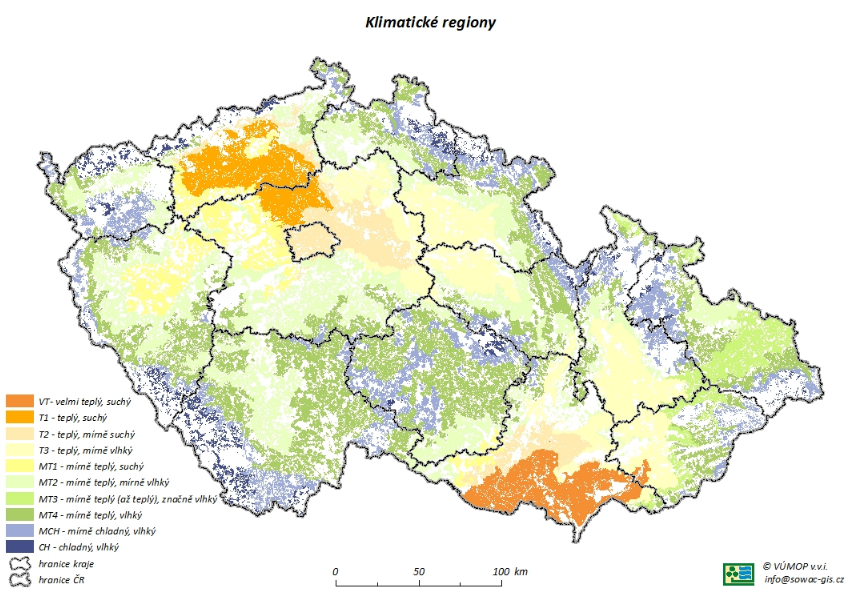
\includegraphics[width=.9\textwidth]{./pictures/klimaticky_region.png}
		\caption[Klimatické regiony]{Klimatické regiony
(zdroj:~\citep{vumop_bpej})}
		\label{fig:klimaticke_regiony}
 	\end{figure}

\subsubsection{Hlavní půdní jednotka}
\label{hpj}

Hlavní půdní jednotka je definována jako účelové seskupení půdních
forem s~příbuz\-nými ekologickými a~agronomickými vlastnostmi. Je
charakterizována genetickým půdním typem, subtypem, půdotvorným
substrátem, hloubkou půdního profilu, zrnitostí a~stupněm
hydromorfismu. V~systému \zk{BPEJ} se uvádí na~druhém a~třetím místě
číselného kódu.

V~současné době systém \zk{BPEJ} vymezuje 78 hlavních půdních jednotek
a~ty jsou dále seskupeny do~13 půdních
typů. Obr.~\ref{fig:klimaticke_regiony} znázorňuje rozložení půdních
typů.

	\begin{figure}[H] \centering
		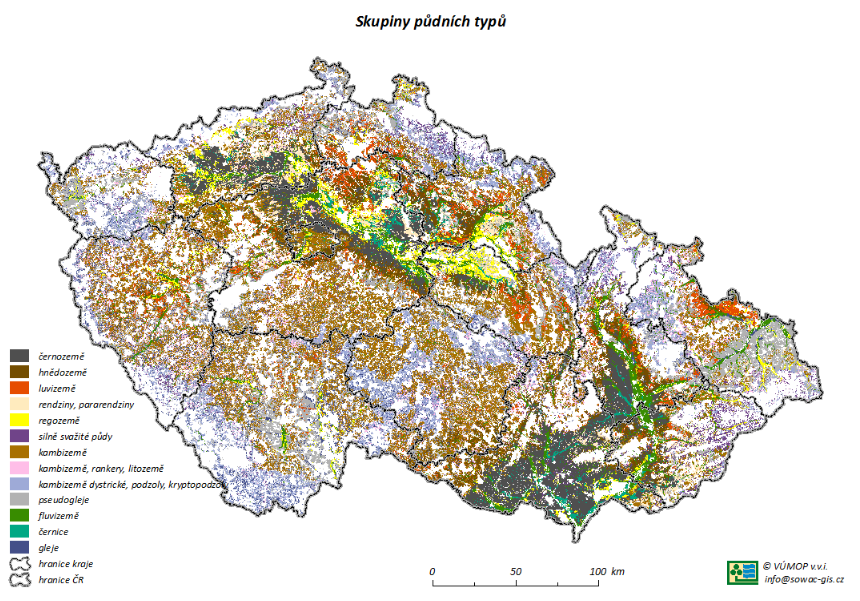
\includegraphics[width=.9\textwidth]{./pictures/pudni_typy.png}
		\caption[Půdní typy]{Půdní typy
(zdroj:~\citep{vumop_bpej})}
		\label{fig:pudni_typy}
 	\end{figure}

\subsubsection{Sklonitost a expozice}
\label{sklonitost_expozice}

Sklonitost se rozděluje do~sedmi skupin. V~terénu se sklonitost určuje
sklonoměrem, jako pomocný podklad lze využít mapy s~podrobným
výškopisem.

Expozice vyjadřuje polohu území \zk{BPEJ} vůči světovým
stranám. V~klimatických regionech \texttt{0}, \texttt{1}, \texttt{2},
\texttt{3}, \texttt{4} a~\texttt{5} se jižní expozice samostatně
hodnotí jako negativní, zbývající expozice se slučují
bez~rozlišení. Samostatně se severní expozice v~klimatických regionech
\texttt{6}, \texttt{7}, \texttt{8}, \texttt{9} uvažuje jako negativní,
expozice východní, západní a~jižní se hodnotí jako sobě
rovné. Expozice se dělí na~čtyři kategorie.

Výsledná třetí číslice kódu \zk{BPEJ} vznikne kombinací sklonitosti
a~expozice~\citep{vyhlaska_327}.

\subsubsection{Obsah skeletu a hloubka půdy}
\label{hloubka_pudy_obsah_skeletu}

Obsah skeletu závisí na~obsahu kamene (pevné částice nad 30 mm)
a~štěrku (pevné částice hornin od~4~do~30~mm), je rozdělen do~čtyř
kategorií.

Hloubka půdy je dána částí půdního profilu omezeného silnou
skeletovitostí, nebo pevnou horninou. Ve~vyhlášce~\citep{vyhlaska_327}
jsou definovány tři kategorie hloubky půdy.

Na pátém místě číselného kódu \zk{BPEJ} se uvádí kód kombinace obsahu
skeletu a~hloubky půdy~\citep{vyhlaska_327}.
